\documentclass[a4paper,11pt,notitlepage]{report}

\usepackage[utf8]{inputenc}
\usepackage{amsmath}
\usepackage{listings}
\usepackage[hidelinks]{hyperref}
\usepackage{catoptions}
\usepackage[left=0.8in, right=0.8in, top=0.8in, bottom=0.8in]{geometry}
\usepackage{color}
\usepackage{soul}
\usepackage{float}
\usepackage{framed}
\usepackage[sc]{mathpazo}
\linespread{1.20}         % Palatino needs more leading (space between lines)
\usepackage[T1]{fontenc}
\usepackage{microtype}
\usepackage{enumerate}
\usepackage{courier}
\usepackage{graphicx}
\usepackage{enumitem}
\usepackage{lipsum}
\usepackage{tikz}
\usepackage{caption}
\usepackage{subcaption}
\usepackage{verbatim}
\usetikzlibrary{shapes,arrows}

\graphicspath{ {./Images/} }

\pdfinfo{
  /Title    (Building Serious Games - Design4Health)
  /Author   (Ralf Nieuwenhuizen, David Prihoda, Ismini Psuxoula, Arnold Schutter, Shen Shuheng)
  /Creator  (Ralf Nieuwenhuizen, David Prihoda, Ismini Psuxoula, Arnold Schutter, Shen Shuheng)
  /Producer (Ralf Nieuwenhuizen, David Prihoda, Ismini Psuxoula, Arnold Schutter, Shen Shuheng)
  /Subject  (Building Serious Games)
}

% Settings for hyperref package (e.g. wat \autoref en \nameref moeten doen)
\hypersetup{
  colorlinks  = false,
  linkcolor   = [rgb]{0.1,0.1,0.5},
  citecolor   = [rgb]{0.5,0.1,0.1},
  filecolor   = [rgb]{0.1,0.5,0.5},
  urlcolor    = [rgb]{0.1,0.1,0.7}
}

\newcommand{\todo}[1] {\hl{#1}}
\setlength{\parindent}{0cm}

\begin{document}

% Define block styles
\tikzstyle{block} = [rectangle, draw, fill=white!20, 
    text width=7em, text centered, rounded corners, minimum height=4em]
\tikzstyle{blockSmall} = [rectangle, draw, fill=white!20, 
    text width=4em, text centered, rounded corners, minimum height=3em]
\tikzstyle{line} = [draw, -latex']
		
\begin{center}
\vskip 1cm
{\Huge Design4Health \vskip 2mm}
{\Large IN4302TU -- Building Serious Games \vskip 1cm}
{\Huge Game Design \vskip 1cm}

\begin{tabular}{ l l }
\textbf{Ralf Nieuwenhuizen} & ($4080408$) \\
\textbf{David Prihoda} & ($4405951$) \\
\textbf{Ismini Psychoula} & ($4411285$) \\ 
\textbf{Arnold Schutter} & ($4260724$) \\ 
\textbf{Shuheng Shen} & ($4298225$)
\end{tabular} 

\end{center}

%\newpage
%\tableofcontents
%\newpage

\chapter{Game Design}

\section{Design concept}
The concept of the design is an engaging game for which the user needs to perform exercises in order to progress. By executing more and more exercises the user has more possibilities in the game and new challenges will become available. 

\subsection{Game Story}
The game starts with a story. 
\\
\textit{2542 AD. Your uncle was one of the first people to buy land in an unknown planet and decided to turn it into a farm to facilitate the earth’s growing needs of foods. As years went by the farm became very profitable and produced the most sought out products. You were very surprised when you received a mail saying that your uncle had left you the farm years ago but you only heard of it now. After so many years, the fields on planet Yeo are unused and empty. Will you be able to salvage the farm? Spend your money wisely to grow the company and unlock new possibilities by doing the exercises.}

\subsection{Gameplay}
The game is about a farm and the user is the farmer. By growing crops and keeping livestock the farmer can grow the company and make money. However, crops and livestock are only available when certain skills are available. To show certain skills, the farmer has to execute exercises in real-life. An exercise is specific for each crop or livestock. For example, the skill for picking apples has to be shown before the apple trees can be bought. 
\\\\
After showing a certain skill, the belonging crop or livestock is unlocked so it can be bought. However, things can only be bought when the farmer has sufficient money, space and energy. The amount of energy represents the time and energy of the farmer during one day. This amount is fixed at the beginning, but can be increasing by becoming more active, or by hiring partners or buying helpful equipment. The amount of space around the farm is fixed throughout the duration of the game. While the game progresses, some old crops or livestock might be sold to free space for new options.
\\\\
The farmer can make money by selling products on the market. Crops should be harvested first, this is done by executing the corresponding exercises for the specific crop. Gaining products from livestock such as milk from the cow also requires the execution of exercises before it is available to be sold. Preparing and selling products on the market also takes energy.
\\\\
During the game, the farmer is allowed to buy machinery or equipment to enlarge the available amount of energy during the day. The extra energy is however only available when an exercise, corresponding to the specific item, is performed during the day. For example, when a pump is bought and this gives $10$ extra energy, the farmer should do the pumping exercise to gain the $10$ extra energy for that day. 
\\\\
Every now and then the farmer receives a special order or task. This can be for example the delivery of specific crops or products within a given time period. When the farmer completes these tasks, the game will advance to the next level. A new level introduces new crops, livestock and equipment.
\\\\
When the exercises are performed sensors are used to measure the movements along with sounds and visualizations to increase the interactivity of the game and make the experience fun.
\\\\
The image below shows all the components in a diagram. (figure~\ref{fig:gameconcept})

\begin{figure}[h]
	\centering
		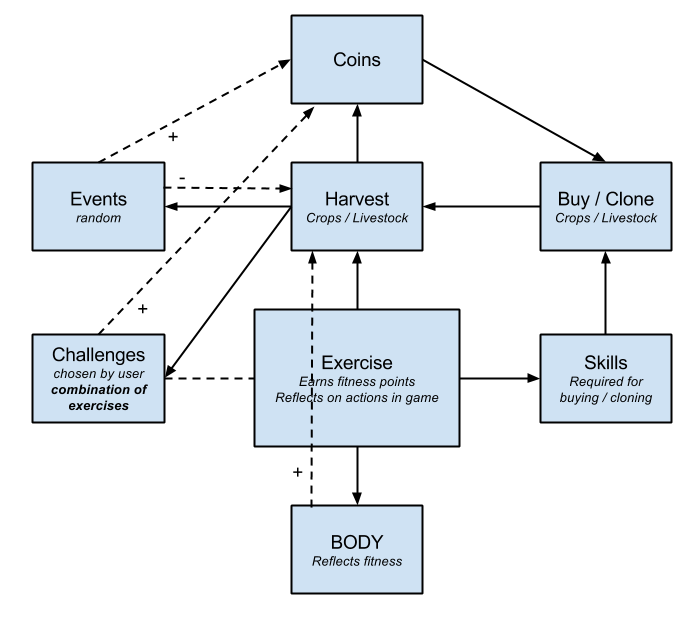
\includegraphics[width=0.80\textwidth]{Images/gameconcept.png}
	\caption{Component diagram of the game}
	\label{fig:gameconcept}
\end{figure}

\section{Extended game design}
In the sections below there is an extended description of all the game features and their specifications. The sections with a star are added on our wishlist, but they will most likely not appear in this prototype.
\subsection{The start}
At the start of the game, the player will be presented with the introducing story, and then he will see his farm. A small explanation of the game will be given, and then the player is ready to start his adventure.
\subsection{The farmer}
In the game, the player will be impersonated by a farmer. This farmer will perform all the real-time tasks the player performs on screen, by which the farmer also gets fitter. During the game, the farmer and the player will become best friends.
\subsection{Exercises}
During the game, players will be confronted with several exercises, which they will have to perform in real life. These exercises will allow them to unlock new crops or tools, or to perform a task in-game, like milking the cows. Before each exercise a clear explanation will be shown on what movement the player has to perform with the phone in hand, demonstrated by a drawing of the farmer. Sensors used: Accelerometer, Gyrometer.

\subsubsection{List of exercises}
\begin{itemize}
\item Alternating stretching arms upward (pick fruit from the tree)
\item Alternating stretching arms bowing down (pick potatoes from the ground)
\item Making circles with arms (harvest crops from circular plant)
\item Swimming movement with arms (fishing)
\item Waving arms backwards and forwards (fishing)
\item Moving hands while sitting in cross-legged position with straight back (milk the cow)
\end{itemize}
\subsection{Energy}
Energy reflects the amount of tasks that can be done by the farmer at one day. Each task that is  performed will cost some energy, so the player will have to decide carefully which tasks he will do first. The amount of energy that a task costs will vary per task. Planting crops, for example, will cost more energy than feeding the chickens. The daily amount of energy can be expanded by hiring Yeomen, the local inhabitants of planet Yeo. Another way to expand the energy is by buying tools, for example a pump to get water faster, or a plowvercraft to plow the fields faster. As the farmer gets more fit, which can be achieved by doing more physical work and exercises each day, energy also increases.

\subsubsection{List of initial farming tools*}
\begin{itemize}
\item Spade
\item Pitchfork
\item Rake
\end{itemize}
\subsection{Money}
When the game begins the player is given a 1000 coins to start developing his farm. After that first allowance he can earn more money by selling his products on the market.
\subsection{Growing crops}
Each type of crop has a name, a cost, a revenue that it brings in when harvested, the time it takes for it to grow. Plants will only last one harvest and have to be harvested soon enough (e.g. two times its growth time), or they die. Trees can last multiple harvests.
\subsubsection{List of crops (cost, time to grow, revenue of single harvest, number of harvests)}
\begin{itemize}
\item Wheat (5, 20, 8, 1)
\item Tomato plant (10, 20, 15, 1)
\item Apple tree (50, 60, 30, 5)
\item Potato plant (30, 60, 40, 1)
\item Yeogrenade plant (50, 50, 60, 1)
\item Carrot plant (30, 30, 40, 1)
\item Pear tree (80, 80, 40, 10)
\item Spacewheat (120, 120, 150, 1)
\item Zorganic melons (300, 240, 500, 1)
\end{itemize}

\subsection{Raising livestock}
Each type of livestock has a name, a cost, a revenue it brings when gathered and the time it takes for it to be ready (for example milking a Milkatron every 8 hours will produce 2 buckets of milk that can be sold for 40 coins each).

\subsubsection{List of livestock}
\begin{itemize}
\item iBeef
\item Milkatron
\item Woolybot
\item Polychick
\item Metagoat
\item Piggium
\item Unicorn
\end{itemize}

\subsection{Advanced Exercises}
Exercises can specifically be designed by physiotherapists for certain physiotherapeutic problems, so these exercises are very useful for certain users. By having these users execute the exercises, that apply to their injury, in the game, they follow a special training program without even noticing. 

\section{Wishlist*}
\subsection{My Store*}
Any product that is finished in the task can be sent to “My Store” (which can be located on another planet), in which you can sell the products. The products can be many different things, for example, coconut milk, apple pies, wool doll, egg pudding, strawberry ice-cream, blueberry pancake, caviar, sushi rolls, etc. Once a product is sold, the corresponding amount of coins will be added to your property.
\subsection{Market*}
Market is somewhere you can buy tools, equipment or any other stuff you might need to fulfill the tasks. For examples see the list below.

\subsubsection{List of tools}
\begin{itemize}
\item a fishing pole (for fishing)
\item a plowvercraft to plow the land
\item a pair of scissors to cut the wool from the sheep (for making the wool doll)
\item a blender to produce juice (for making fruit ice-cream)
\item a flour mill to grind the wheat (for making dough)
\item an oven to bake stuff (for making cakes)
\item a rice cooker to cook rice (for making sushi rolls)
\item fertilizer for the crops (for gaining more crops each season)
\item a harvestroid to reap the crops (for saving your energy)
\item a pump to get easier access to water
\item a warpsaw to cut the trees
\end{itemize}
\subsection{Tasks*}
Every now and then the farmer receives a special order or task. This can be for example the delivery of specific crops or products within a given time period. When the farmer completes these tasks, the game will advance to the next level. A new level introduces new crops, livestock and equipment.

\subsubsection{List of tasks}
\begin{itemize}
\item Bake an apple pie for your sick neighbour Yeowoman.
\item Make a wool doll for your cousin as a birthday present.
\item Prepare sushi rolls for the picnic with your friends.
\item Make strawberry ice-cream for Hawaii party.
\item Save the farm from an attack of neighbouring Aliens (antagonists).
\end{itemize}

\section{Use cases / interactions}
Example: Bake an apple pie and sell it.
\begin{enumerate}
\item Do exercise to unlock the apple tree
\item Do exercise to unlock the wheat
\item Grow the apple tree and the wheat
\item Harvest the apple tree and the wheat by doing related exercise
\item Go to the market to buy the oven and flour mill*
\item Bake the apple pie*
\item Send it to “My Store” and sell it *
\item Earn the corresponding amount of coins
\end{enumerate}

\section{Phases}
Here we type an overview of which parts of the game will be ready in what phase
\subsection{Designing the game}
Before starting on developing the actual software, there will be sketches for all screens of the game, to create a clickable static prototype. This will be presented to the group, and after that final decisions are made on the design.

\subsection{First playable}
The first playable will be a small version of the final game. It will not be as complete, but the vital functions will be there, for example the farm, some sort of crop, the money, place and energy, and some livestock. There will be some user tests and the progress will be reported to the commissioners.
\subsubsection{Week 3}
\begin{itemize}
\item Combine first playable with sensors
\item Make the view scalable
\item First design of the farm’s view
\item Build designs for the basic stuff in the game (pick at least one from each group).
\end{itemize}
\subsubsection{Week 4}
\begin{itemize}
\item Energy
\item Money
\item Have an exercise in-game
\item Have a crop working in-game
\item Have one type of livestock working in-game
\end{itemize}
\subsection{Beta version}
The beta version will already have all of the main features of the final game. Most of the crops and livestock will be buildable and money and energy will work perfectly. The beta version will be tested on the target audience.
\subsubsection{Week 5}
\begin{itemize}
\item Complete the functionalities of the gameplay (energy/money/exercises)
\item Build models for all crops, livestock, menu items
\item User testing
\end{itemize}

\subsubsection{Week 6}
\begin{itemize}
\item Complete list of crops in-game
\item Complete list of livestock in-game
\item Implement changes from user tests
\end{itemize}
\subsection{Final version}
In the final version we will have added all the features from the list above, and maybe even some from the wishlist(*). The game will again be tested on the target audience.
\subsubsection{Week 7}
\begin{itemize}
\item Fix bugs / Finetuning
\item Wishlist
\end{itemize}
\subsubsection{Week 8}
\begin{itemize}
\item Write report
\item User testing
\end{itemize}

\section{Requirements}
\subsection{Changed requirements from the commissioners}

\subsection{Target audience}
The envisioned design will fulfill the requirement of being an engaging, activating game. This is all meant to activate people while doing an activity they love, gaming. As there are no real age requirements, an age group will be set as soon as we determine how complex the game will be. Adding features to the farm will make the game more appropriate for older people (think of people over $12$ years), and keeping it simple will keep the target age group a little younger (more like $8$-$14$ years). The game will be serious, as there is a clear purpose behind it of activating people, and it will be fun, as is proven by previous games in which you build up your own world, and have to show dedication to keep it up and running.

\subsection{Resources}
To get from a paper prototype to a full up and running game some resources will be needed. Because it will be a smartphone application, no external sensors will be needed. Plenty of open source software is available to fulfill our needs. The only cost we will have is the Android Developer registration fee which is \$25.
\subsubsection{Hardware}
The only requirement for someone to play our game will be that he owns a smartphone. Research about the sensors on each phone we can use will be done. Most likely these will include the accelerometer, GPS, and microphone.
\subsubsection{Software}
The game will be developed for Android mobile phones, using open source software. 
We will most likely go for HTML5 supported by javascript, eventually with supporting libraries. The HTML5 can be converted to a native app by using PhoneGap (\url{http://phonegap.com/}). This also gives us the option to convert to other mobile platforms, like iOS and Windows (Phone)

\section{Testing plan}




%\bibliography{synopsis}
%\bibliographystyle{plain}

\end{document}
